\documentclass[conference]{IEEEtran}
\IEEEoverridecommandlockouts
% The preceding line is only needed to identify funding in the first footnote. If that is unneeded, please comment it out.
\usepackage{cite}
\usepackage{amsmath,amssymb,amsfonts}
\usepackage{algorithmic}
\usepackage{graphicx}
\usepackage{textcomp}
\usepackage{xcolor}
\usepackage{lipsum}
\usepackage{hyperref}
\hypersetup{
    colorlinks,
    linkcolor={black},
    citecolor={black},
    urlcolor={blue!80!blue}
}

\def\BibTeX{{\rm B\kern-.05em{\sc i\kern-.025em b}\kern-.08em
    T\kern-.1667em\lower.7ex\hbox{E}\kern-.125emX}}
\begin{document}

\title{DeepRob Final Project Report:\\NeRF Supervision: Learning Dense Object Descriptors from Neural Radiance Fields
}

\author{\IEEEauthorblockN{Manu Aatitya Raajan Priyadharshini}
\IEEEauthorblockA{\textit{Robotics} \\
\textit{University of Michigan}\\
Ann Arbor, USA \\
rpmanu@umich.edu}
\and
\IEEEauthorblockN{Rohit Banerjee}
\IEEEauthorblockA{\textit{Robotics} \\
\textit{University of Michigan}\\
Ann Arbor, USA \\
rohitban@umich.edu}
\and
\IEEEauthorblockN{Aravind Krishnakumar}
\IEEEauthorblockA{\textit{Robotics} \\
\textit{University of Michigan}\\
Ann Arbor, USA \\
karavind@umich.edu}
}

\maketitle


\begin{abstract}
In this paper, we present NeRF Supervision \cite{yen2022nerfsupervision} - a technique for learning dense object descriptors from Neural Radiance Fields. In this project, we discuss about NeRFs as a 3D reconstruction tool to model shiny and reflective surfaces to generate better reconstruction and to train dense correspondences for manipulation of such objects.  
% \lipsum[1]
% The project page is available at: \href{https://deeprob.org}{https://deeprob.org}.
The Github project page is available at: \href{https://github.com/manuaatitya/rob599-final-project}{DeepRob Project}
\end{abstract}

\section{Introduction} 

Non-Lambertian common household objects, such as forks or whisks, are challenging to manipulate since traditional photogrammetry techniques fail to model such objects accurately. These objects have a high degree of reflectivity and tend to reflect light in a highly directional manner, making it difficult to capture their surfaces precisely, as shown in Fig (\ref{fig:fork_colmap}). Similar to COLMAP, multi-view stereo (MVS) also fails to produce an accurate depth map that can be used to reconstruct highly specular materials or objects \cite{yen2022nerfsupervision}. Therefore, the primary motivation to reconstruct visual descriptors for highly-specular materials such as forks is due to the difficulty in modeling these objects using traditional photogrammetry techniques like MVS or COLMAP.\cite{schoenberger2016sfm}. \vspace{2mm}

\begin{figure} [h]
\centering
  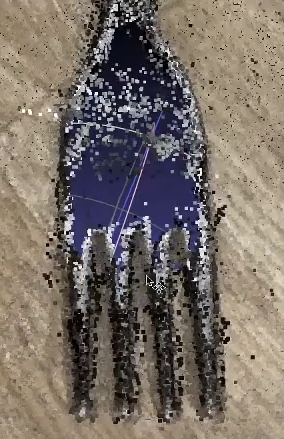
\includegraphics[scale = 0.4]{figures/introduction/fork.png}  
  \caption{\label{fig:fork_colmap} \textbf{Fork COLMAP} Reconstruction attempt from the fork dataset in \cite{yen2022nerfsupervision}. Our initial attempts highlight the issues with COLMAP reconstruction of highly specular objects as it is unable to obtain an accurate depth map}
\end{figure}

It is especially important to model a scale, illumination, and pose invariant descriptor of highly-specular materials when considering robotic manipulation. Most robotic manipulators are equipped with commodity RGB-D cameras or MVS. To address the limitations of traditional stereo techniques and COLMAP, Lin et al. \cite{yen2022nerfsupervision} introduced NeRF supervision for learning dense object-centric dense correspondences - an RGB-only, self-supervised pipeline based on NeRFs.\vspace{2mm}

Neural Radiance Fields (NeRFs) have demonstrated remarkable ability in performing view synthesis on objects with thin structures or reflective properties, which has motivated their use in this domain. NeRF is the state-of-the-art scene representation technique that uses a feed-forward neural network to model a continuous representation of scenes and objects \cite{understanding-nerfs}. Compared to previous methods such as DeepSDF or SRNs, NeRF renderings are better in terms of both qualitative and quantitative performance.

\begin{figure} [h]
\centering
  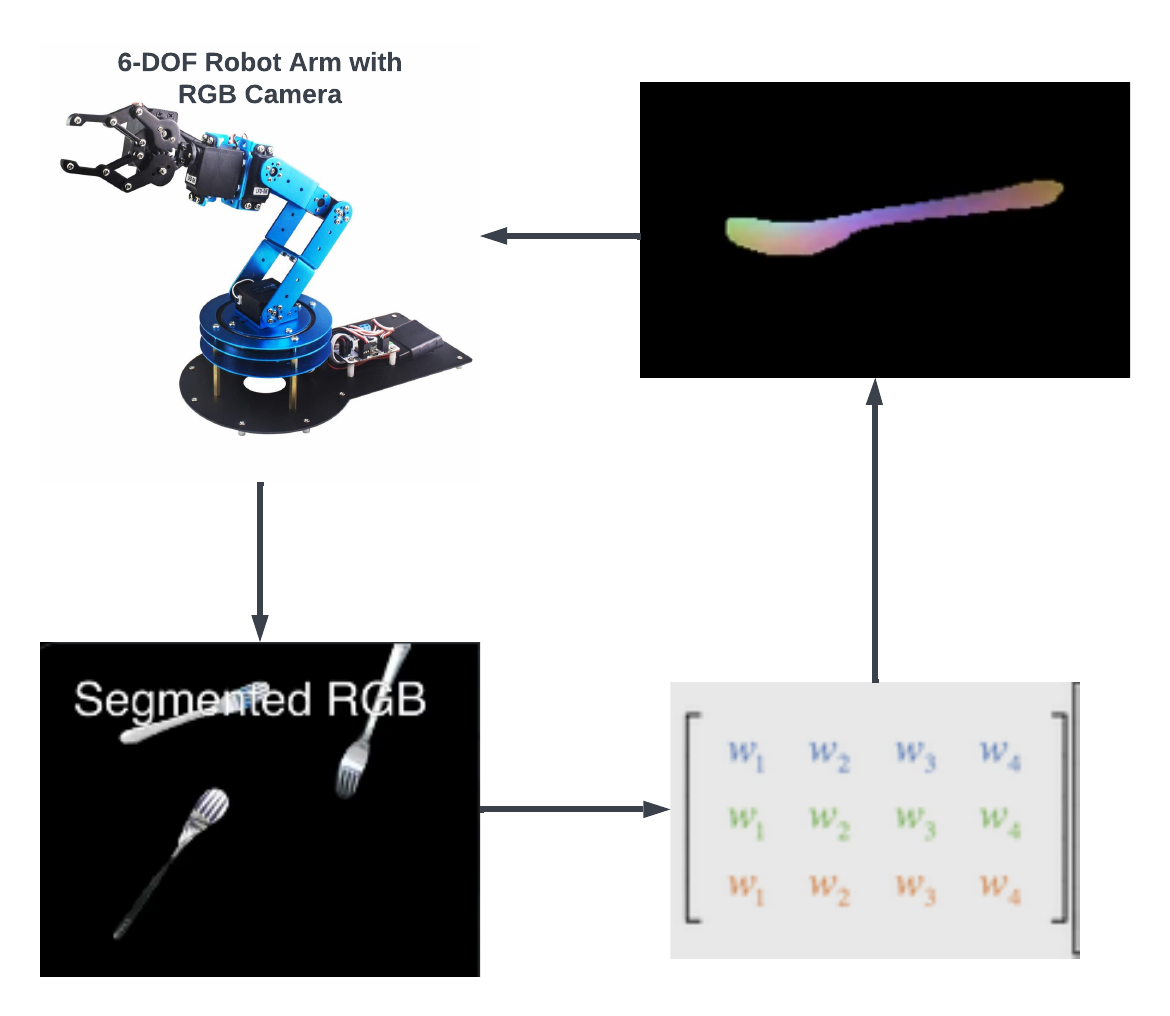
\includegraphics[scale = 0.45]{figures/introduction/flowchart_nerf_supervision.png}
  \caption{\label{fig:Flowchart} \textbf{Flowchart NeRF Supervision} (a) A 6-DOF Robot arm with commodity RGB used for object manipulation, (b) RGB camera used to segment object of interest, (c) Using the semantic label of the segmented RGB + Camera View direction, corresponding weights of the object are used to generate a RGB-D image, (d) The dense correspondence generated by NeRF's allows the modelling of off-the shelf visual descriptors such that the robot arm can grasp the object}
\end{figure}

In the NeRF supervision paper, NeRFs were used to model a scene as input to extract dense correspondences between multiple views. Further, the dense correspondence data was utilized as training data to learn a view-invariant representation of an object \cite{yen2022nerfsupervision} \cite{florencemanuelli2018dense}. This approach has significant implications for object manipulation in robotic systems. As the 3D object scenes of an object are stored as memory-efficient weights, if the robot vision system can identify and segment an object  (RGB), a corresponding view can be reconstructed through NeRF with dense correspondence (enabling pixel matching by RGB between different scenes). Fig (\ref{fig:Flowchart}) illustrates the pipeline of NeRF supervision for object grasping and manipulation at a high level. \vspace{2mm}

This paper provides an overview of the literature reviewed, to successfully reproduce and extend the research. The Methodology section outlines the approach taken in this process, including a detailed explanation of our work. The Results section presents the findings from reproduction and extension, followed by a brief discussion of their implications. Finally, the conclusion and future work for this project are discussed. \vspace{2mm}


\section{Related Work}
\textbf{Neural Radiance Fields.} NeRF is a powerful technique that can reconstruct 3D scenes with remarkable detail and photorealism using 2D images. By using a multi-layer perceptron (MLP) neural network, NeRF can predict the volumetric density and view-dependent RGB color of each point in a 3D space from a single 2D image by regressing from 5D coordinates $(x,y,z,\theta,\phi)$. This information can then be used to render novel views of the scene from any viewpoint. By improving MLP performance with problem-specific Fourier features \cite{tancik2020fourier} and embedding it into a volumetric rendering engine, the resulting MLP achieves mapping of input coordinates to a density field, even for low-dimensional regression tasks. NeRF has shown superior performance in 3D scene reconstruction and novel view synthesis across various datasets. Although NeRF has been mainly used for graphics and vision tasks, it has also shown potential for use in robotics, such as for pose estimation and SLAM. However, using NeRF in a robotics context can pose challenges because it represents all scene content as a volumetric quantity, which does not directly estimate object boundaries or produce depth maps. Nonetheless, the estimated density field by NeRF can be used to synthesize depth maps by calculating the expected depth from a ray, and recent research has been exploring ways to improve these depth maps. \vspace{2mm}

\textbf{Depth-supervised NeRF.} DS-NeRF (Depth-supervised Neural Radiance Fields) \cite{deng2022depthsupervised} proposes a solution to some of the limitations faced by Neural Radiance Field (NeRF), such as producing poor renderings from fitting inaccurate scene geometries due to a small number of input views or taking 10 hours or more to train when given a large number of input views. This is mainly due to a missing constraint that the scene's geometry may mostly comprise empty spaces and opaque objects/surfaces. To address this, DS-NeRF formulates a loss for learning radiance fields by exploring depth as a cheap source of supervision. DS-NeRF follows the current NeRF pipeline, which requires images and camera poses estimated using structure-from-motion (SFM) solvers such as COLMAP or bundle adjustment. DS-NeRF implements the loss function such that the distribution of a ray's depth can match a given 3D keypoint, thus incorporating reprojection error as a depth uncertainty measure. The depth supervision used by DS-NeRF improves NeRF's performance by rendering better images with fewer training views while training faster. \vspace{2mm}

\textbf{NeRF in the Wild.} NeRF-W \cite{nerf_w} proposes a solution to another limitation faced by Neural Radiance Fields, which assumes that the world within each view is geometrically and photometrically static. This means that two views provided to train from the same position and orientation must be identical. This limitation of NeRF causes its performance to decrease when presented with moving objects or variable lighting conditions, thus restricting its application to large-scale-in-the-wild scenarios. NeRF-W addresses this limitation by modeling per-image appearance variations in a lower-dimensional latent space and optimizing its embedding following the framework of Generative Latent Optimization, which relaxes the imposed need for consistency in the photometric and environmental variations between images. Furthermore, NeRF-W allows for the unsupervised decomposition of the scene into static and transient components by modeling the scene as a union of shared and image-dependent elements. This is achieved by using a secondary volumetric radiance field combined with a data-dependent uncertainty field, which reduces the effect of transient objects in a static scene representation. Several challenging in-the-wild photo collections of cultural landmarks were trained using NeRF-W, which produced detailed, high-fidelity renderings from novel viewpoints, surpassing the prior state-of-the-art by a large margin on PSNR and MS-SSIM. \vspace{2mm}

\textbf{Dense Object Nets.} Dense visual descriptors play a crucial role in representing objects and other features for tasks such as 3D scene reconstruction, object-pose estimation, and robot manipulation. Currently, machine-learning approaches are commonly used to train visual descriptors. Dense Object Nets \cite{florencemanuelli2018dense} is a self-supervised framework for learning dense visual object descriptors that can be used for robotic manipulation tasks. The approach is based on training a deep neural network to predict pixel-wise correspondences between images of the same object in different poses, which can be widely applied to a variety of previously unseen and non-rigid objects. The network architecture used in Dense Object Nets is a Siamese architecture. In this architecture, two images of an object are fed into two identical branches of the network, and the objective is to minimize the L2 distance between the feature maps produced by the two branches. The resulting dense object descriptor can be used for tasks such as object recognition, pose estimation, and grasping, primarily due to its ability to generalize across a class of objects. Dense Object Nets outperforms state-of-the-art methods on several benchmark datasets such as GLU-Net, GOCor, and PDC-Net. Moreover, it has been demonstrated to work well on real-world robotic manipulation tasks. \vspace{2mm}

\section{Methodology and Algorithmic Extension}

Our approach for reproduction and extension of the paper required an understanding of the theoretical background and code of NeRF-supervision \cite{yen2022nerfsupervision}, Dense Object Nets \cite{florencemanuelli2018dense} and DS-NeRF \cite{deng2022depthsupervised}.

\subsection{Theoretical Background}

\textbf{Depth-Supervision and NeRF-Supervision} - 
The architecture of NeRF is the same between DS-NeRF and NeRF-Supervision. The only change made in NeRF-Supervision was the modification of the loss function to account for RGB pixel correspondence. In Fig. (\ref{fig:Nerf_Architecture}), a multi-layer perceptron (MLP) feed-forward architecture is provided, where the width and height of the hidden layers are 256 and 8, respectively.
    
\begin{figure} [h]
\centering
     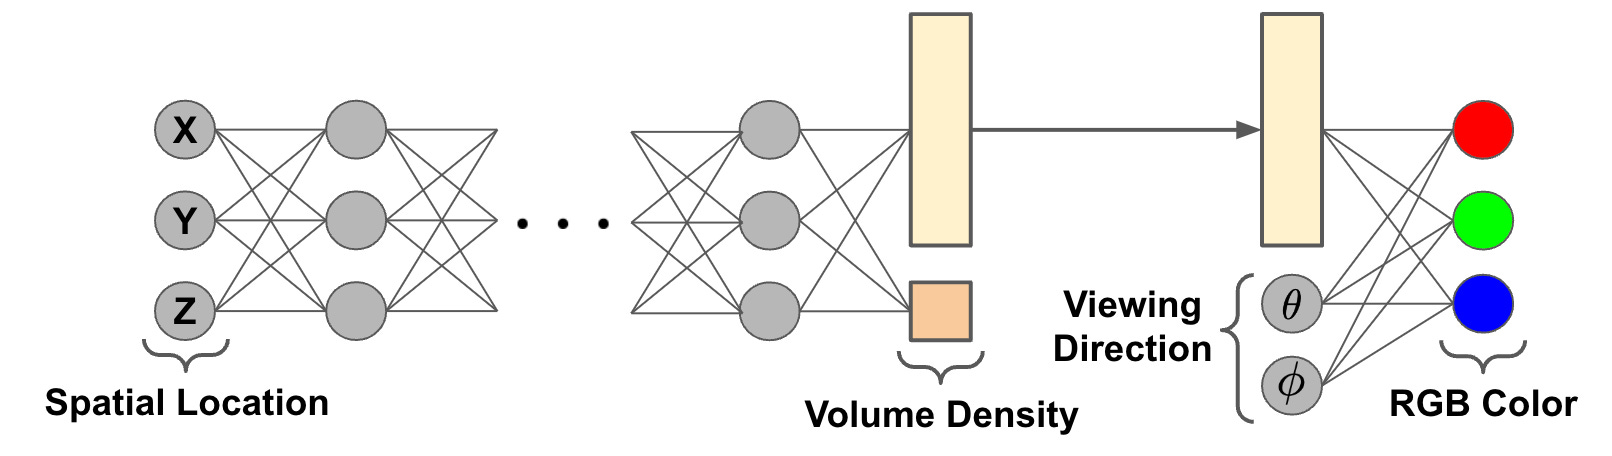
\includegraphics[scale = 0.15]{figures/Method/Nerf_architecture.jpg}
     \caption{\label{fig:Nerf_Architecture} \textbf{Feed-forward architecture of DS-NeRF and NeRF-Supervision}}
\end{figure}

The inputs to the 8-layer MLP are the (x,y,z) spatial coordinates, which are then embedded to a higher-dimensional space using high-frequency Fourier functions \cite{tancik2020fourier}. The length of the embedding is a hyperparameter set to 10 for both DS-NeRF and NeRF-Supervision. To avoid vanishing gradient issues, the input spatial coordinates are passed to the fourth layer of the MLP. The output of the MLP is a feature vector of width 256 and volume density, which is a 1x1 vector.
\vspace{2mm}

The feature vector is sent through another MLP layer, which is concatenated with the viewing direction. The viewing direction is also embedded in a higher dimension using Fourier analysis, with the length being the same as that of the spatial coordinates. The output of this final layer is the RGB values corresponding to the spatial coordinates and viewing direction.
\vspace{2mm}

\textbf{Dense Object Descriptors} -  For each pixel $\in \mathbb{R}^{W x H x 3}$, a descriptor of size $\mathbb{R}^{W x H x D}$ is mapped, which describes the local surroundings around the pixel location, where D is the dimension of the descriptor (typically in the order of 128).

These D-dimensional vectors are trained in a \textbf{Siamese} fashion, where a pair of RGB images are taken and verified for a match by checking if they are in the same vertex in the 3D reconstruction. A neural network is trained to learn this pixel-to-pixel correspondence. The images are split into two batches of \textbf{matches} and \textbf{non-matches}, where matches refer to the images that have a pixel correspondence, and non-matches refer to the pixels that don't have a pixel correspondence. The loss function is trained to \textbf{minimize the matches loss} and \textbf{maximize the non-matches loss}. \vspace{2mm}

Since the dense object descriptors require a good 3D reconstruction of the object for learning, NeRFs have been used in the main paper \cite{yen2022nerfsupervision} to create a good 3D rendering of the object.

\subsection{Code Reproduction}

The reproduction of the NeRF Supervision code had multiple dependencies that needed to be satisfied to be able to reproduce the code successfully. The following steps need to be performed to get NeRF-Supervision or DS-NeRF working: 

\begin{enumerate}
    \item Install COLMAP with the required dependencies as stated in the COLMAP library \cite{schoenberger2016sfm}.
    \item Run the .py file "img2poses" which internally runs COLMAP to generate the ground truth depth, hierarchical pairing of similar images (important for the NeRF algorithm to work), and a homogeneous matrix containing the rotation matrix and translation vector.
    \item The "train\_nerf" function as stated in the GitHub repository can be run on the terminal to start training the NeRF. The original code provided seemed to have multiple bugs which we fixed to get the algorithm to start training. The changes made were as follows:
    
    \begin{enumerate}
        \item The "minify" function, which resized the images by a factor of 8, had to be rewritten to get it working.
        \item Certain variables had to be moved to "cuda" between various functions.
        \item Generation of certain folders needed to be changed/deleted to enable COLMAP wrapper to run successfully.
    \end{enumerate}

    \item Finally, post-training, the "render\_nerf" command needs to be run to get the final outputs and the log files. The completion of this step completes the reproduction of the NeRF algorithm.
    \item To generate the dense object descriptors, the PyTorch dense correspondence repo had to be run using docker.
    \item The docker image needs to be run in a virtual environment to install the required libraries with older versions of the libraries used to generate dense object descriptors.
    \item To successfully run the docker image, we had to divide the image into two separate images, which have been added to the Docker Hub to enable easier reproduction of this part of the code.
    \item Nvidia drivers for the correct CUDA versions had to be installed.
    \item Post this, dense object descriptors can be run in Jupyter notebooks using the examples given in the original code.
\end{enumerate}

Our team was successful in reproducing both papers, and results from our reproduction can be found on our \href{https://github.com/manuaatitya/rob599-final-project/tree/master/nerf-supervision-public/logs/fork}{Github} as well as \href{https://hub.docker.com/r/manuaatitya/pytorch-dense-correspondence}{Docker Hub}. Unfortunately, we were unable to attach the results of the visual descriptors we generated from the Dense Object Nets paper \cite{florencemanuelli2018dense} to this report, as we did not store the data due to some technical issues.

\subsection{Difficulties Encountered:}
\begin{enumerate}
    \item Since the training required around 200,000 iterations to train the NeRFs for reconstructing the scene, it was very difficult to train the network without any powerful local Nvidia GPU. The code has a tensorRT dependency due to which we were unable to run the pipeline on Colab or Colab Pro.
    \item There were very little instructions on the NeRF code itself and certain functions like minify took us multiple days to process through and debug.
    \item The pytorch-dense-correspondence \cite{florencemanuelli2018dense} repository contains code written in Python 2 with many deprecated dependencies, which needed significant changes to the code. Eventually, a new docker image with all the required dependencies to test the code off the shelf was created as part of the reproduction process and uploaded to \href{https://hub.docker.com/r/manuaatitya/pytorch-dense-correspondence}{docker-hub}.
\end{enumerate}

\section{Experiments and Results}
The GitHub code \cite{yen2022nerfsupervision} was successfully reproduced with changes made to specific functions of the code.
% This section should describe the experimental design and associated results that are used to analyze the algorithmic extension. This section my be broken up into subsections such as:

\subsection{Reduced Training Set Images}
The NeRF was trained using only half the number of images in the test dataset, and the results were compared with the original reproduction presented in the NeRF-Supervision paper \cite{yen2022nerfsupervision}. The PSNR value for the reproduced results was 31, and the loss was 5e-4. Additionally, a realistic render of the fork was generated, as seen in Fig [\ref{fig:fork_result}]. These results demonstrate that the proposed architecture can produce considerable results even with fewer training images than what was used in the original work \cite{yen2022nerfsupervision}.

\begin{figure} [h]
\centering
  
\includegraphics[scale = 0.55]{figures/results/fork-result.png}  
  \caption{\label{fig:fork_result} Fork Colmap Reconstruction}
\end{figure}

% The design of each experiment should be described such that the results are reproducible for a reader (i.e. which datasets are used, how are the metrics defined, which hyperparameters were used, etc.).
% \lipsum[13]

\subsection{Segmented Images}
Instead of the complete image as the input for the NeRF, a segmented image using pre-trained Segment Anything with the ONNX Model \cite{kirillov2023segment}, was generated as shown in Fig [\ref{fig:fork_seg}] where  the forks were segmented to extract just the object and darken the background for use as input to the NeRFs. The motivation behind this approach is to reduce the width of the NeRF MLP from 256 to 128, to see if it could learn the scene with fewer parameters in the MLP, that would help to reduce the training time considerably.

\begin{figure} [h]
\centering
  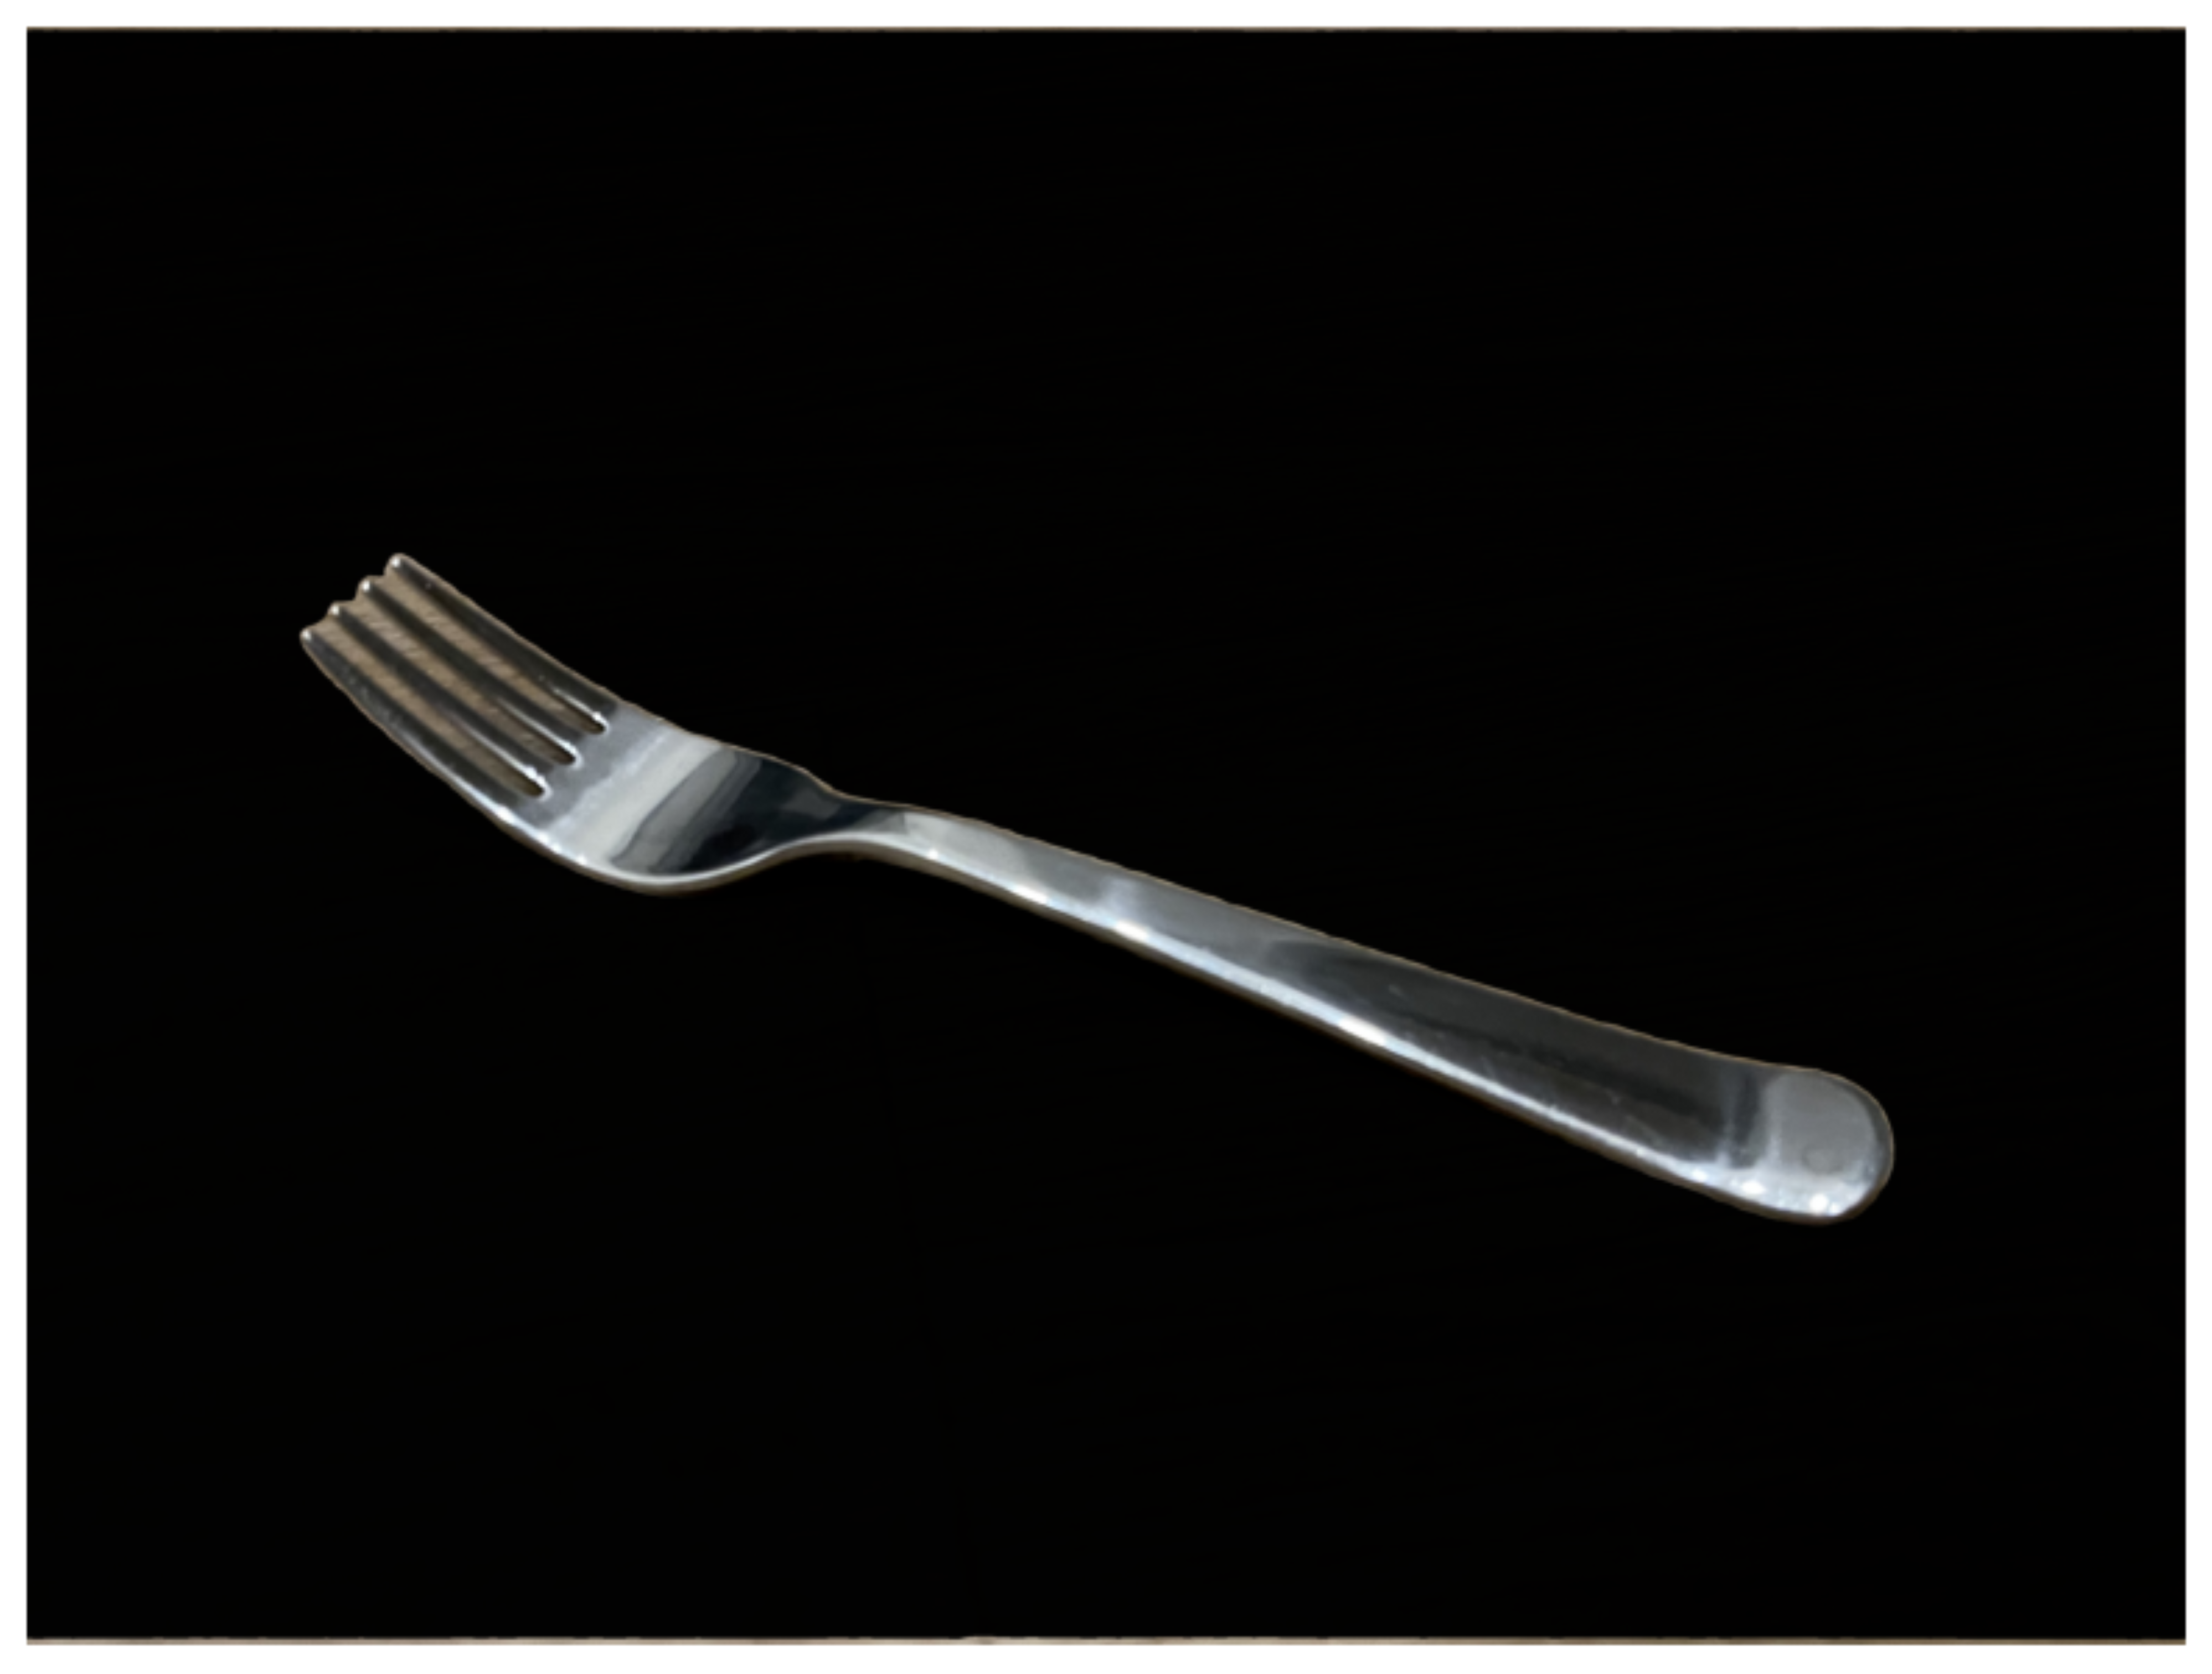
\includegraphics[scale = 0.07]{figures/results/fork-segment.png}  
  \caption{\label{fig:fork_seg} Segmented Fork Image}
\end{figure}

We encountered some challenges that prevented us from testing our final hypothesis. One of these was the loss of meta-data during image segmentation, but we were ultimately able to address this issue with considerable effort. However, we were not able to test our hypothesis fully because COLMAP failed on these images. The software did not have enough information to perform hierarchical sampling or pair similar images together due to the low number of features in these images.

% The results that were observed should be described in this section.
% \lipsum[14]

\subsection{Effect of Embedding Layer Transformation} \label{hyper-parameter-section}
One of the key steps in the NeRF pipeline is passing the input images to a higher dimensional embedding layer that encodes the data from x, y, and z positions to higher dimensional vectors using Fourier series representation of the radiance signal along the ray. This is an important hyperparameter in tuning the NeRFs as the positional encoding layer is the one that decides between a feature-rich realistic render and a normal render. However, the motivation for the choice of this hyperparameter referred to as 'multires' is not mentioned in the code or the paper. A default value of 10 (units of $log_2$) has been chosen. When tried with the custom shoe dataset, it was observed that increasing this hyperparameter gave a significant increase in the Peak Signal to Noise Ratio (PSNR) values, as seen in the results in Table [\ref{table:1}].

\begin{table}[h!]
\centering
\begin{tabular}{ |p{2.5cm}|p{2cm}|p{2cm}|  }
 \hline
 \multicolumn{3}{|c|}{PSNR Analysis} \\
 \hline
 multires parameter ($log_2$ scale) & PSNR start & PSNR End \\
 \hline
 10  & 13.4    & 17.8 (200,000) iterations \\ \hline
 50  &   14.1  & 18.1 (50,000 iterations) \\
 \hline 
\end{tabular}
\vspace{2mm}
 \caption{PSNR Analysis Results}
\label{table:1}
\end{table}

Although the model was observed to overfit with more weight matrix elements when using 50 as the \textit{multires} parameter, the PSNR value significantly increased, indicating that the reconstruction was considerably better than with the original parameter.

\subsection{Deformable and Occluded Object Modeling}
Another hypothesis that needed verification was whether the current NeRF architecture could be used for reconstructing deformable and occluded objects. To test this, a custom dataset of a shoe with slight deformations and partial occlusions from certain viewing directions was used as input for the NeRF model, and the results were analyzed. However, the reproduction results were not as good as those for rigid object modeling, as seen in Fig [\ref{fig:shoe}].

\begin{figure} [h]
\centering
  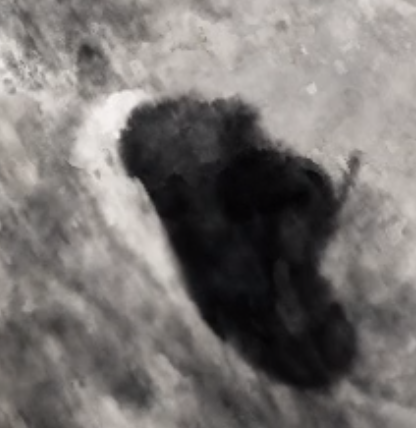
\includegraphics[scale = 0.35]{figures/results/shoe.png}  
  \caption{\label{fig:shoe} Reconstructed Shoe Image}
\end{figure}

\subsection{Training / Compute Analysis:}
One of the important aspects left out in the main paper \cite{yen2022nerfsupervision} is the computational resources and the training time required to fully train the model. When tested on multiple host systems, the following are the resources required for the training process.

\begin{table}[h!]
\centering
\begin{tabular}{ |p{2.5cm}|p{2.3cm}|p{2.5cm}|  }
 \hline
 \multicolumn{3}{|c|}{Compute Time Analysis} \\
 \hline
 System Specifications & Training Time (hrs) & Number of iterations \\
 \hline
 16 GB RAM with 8 GB 1660 GTx GPU  & 46 & 200,000 \\ \hline
 16 GB RAM with 16 GB 1660 GTx GPU  & 24 & 200,000 \\ \hline
 128 GB RAM  with 64 GB 1660 GTx GPU &   10  & 200,000 \\
 \hline 
\end{tabular}
\vspace{2mm}
 \caption{Compute Time Analysis Results}
\label{table:2}
\end{table}

Table [\ref{table:2}] clearly shows that the training of NeRFs requires significant computational resources, making it difficult to train even in Google Colab Pro.

\section{Conclusions and Future Work}
In conclusion, based on the results, the following can be inferred:

\begin{enumerate}
\item NeRFs are a good alternative method of representation for rigid object modeling.
\item NeRF supervision MLP architecture requires extremely high-quality images and heavy computational resources for training. Alternate approaches like NeRF-W provide better results for low-quality images.
\item The code can be significantly improved by hyperparameter tuning as demonstrated in Section [\ref{hyper-parameter-section}].
\end{enumerate}

In the future, the following implementations can be considered:

\begin{enumerate}
\item The idea of transient embeddings \cite{nerf_w} could be added to the existing NeRF architecture to improve better reconstructions. Transient embeddings have proven to be lighting invariant and handle occlusions.
\item Pre-processing techniques like segmentation can be used to reduce the MLP model dimensions, which can save considerable training time and resources required for training.
\end{enumerate}


\bibliographystyle{IEEEtran}
\bibliography{biblio}

\end{document}
